\documentclass[main-ap-physics.tex]{subfiles}


\begin{document}

\begin{example}
    \textit{What Rocket Thrust Accelerates This Sled?}\\
    Prior to space flights carrying astronauts, rocket sleds were used to test aircraft, missile equipment, and physiological effects on human subjects at high speeds. They consisted of a platform that was mounted on one or two rails and propelled by several rockets. Calculate the magnitude of force exerted by each rocket, called its thrust $\vec{T}$, for the four-rocket propulsion system shown in Figure \ref{1lc8tY}. The sled's initial acceleration is  \SI{49}{m/s2^}, the mass of the system is \SI{2100}{kg}, and the force of friction opposing the motion is known to be \SI{650}{N}.
\end{example}

\begin{center}
    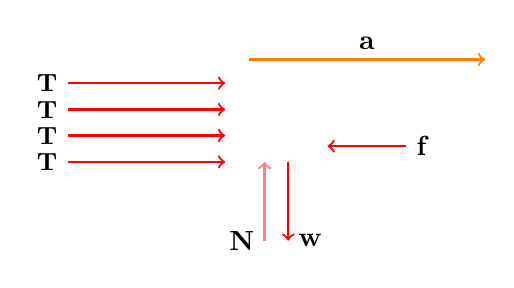
\begin{tikzpicture}
        \node[right] at (0,0) {\HUGE \mysled};
        \pgfplotsinvokeforeach{-1*0.5,-0.33*0.5,0.33*0.5,1*0.5}{
            \draw[thick,red,->] (-2,#1) node[left,black] {\small \textbf{T}} -- ++(2,0) ;
        }
        \draw[->,thick,red!50] (0.5,-1.5) node[left,black] {\textbf{N}} -- ++(0,1);
        \draw[<-,thick,red] (0.8,-1.5) node[right,black] {\textbf{w}} -- ++(0,1);
        \draw[->,thick,orange] (0.3,0.8) -- ++ (3,0) node[above,black,pos=0.5] {\textbf{a}};
        \draw[->,thick,red] (2.3,-0.3) node[right,black] {\textbf{f}} -- ++(-1,0);
    \end{tikzpicture}

    \vspace{1em}
    
    \begin{tikzpicture}
        \node at (2,2) {Free-body diagram};
        \fill[red] (0,0) circle (2pt);
        \draw[->] (-0.1,0) -- (-0.6,0) node[left] {\textbf{f}};
        \draw[->] (0,0.1) -- ++(0,1) node[above] {\textbf{N}};
        \draw[->] (0,-0.1) -- ++(0,-1) node[below] {\textbf{w}};
        \pgfplotsinvokeforeach{0.1,1.7,3.3,4.9}{
            \draw[->] (#1,0) -- ++(1.5,0) node[above,pos=0.5] {\textbf{T}};
        }
    \end{tikzpicture}
    \captionsetup{type=figure,margin=1in,font=scriptsize}
    \captionof{figure}{A sled experiences a rocket thrust that accelerates it to the right. Each rocket creates an identical thrust \textbf{T}. As in other situations where there is only horizontal acceleration, the vertical forces cancel. The ground exerts an upward force \textbf{N} on the system that is equal in magnitude and opposite in direction to its weight, \textbf{w}. The system here is the sled, its rockets, and rider, so none of the forces between these objects are considered. The arrow representing friction (\textbf{f}) is drawn larger than scale.}
    \label{1lc8tY}
\end{center}

\Solution \textit{Strategy}: Although there are forces acting vertically and horizontally, we assume the vertical forces cancel since there is no vertical acceleration. This leaves us with only horizontal forces and a simpler one-dimensional problem. Directions are indicated with plus or minus signs, with right taken as the positive direction. See the free-body diagram in the figure.

\vspace{1em}

Since acceleration, mass, and the force of friction are given, we start with Newton's second law and look for ways to find the thrust of the engines. Since we have defined the direction of the force and acceleration as acting ``to the right,'' we need to consider only the magnitudes of these quantities in the calculations. Hence we begin with

\begin{equation*}
    F_{\text{net}} = m a
\end{equation*}

where $F_{\text{net}}$ is the net force along the horizontal direction. We can see from Figure \ref{1lc8tY} that the engine thrusts add, while friction opposes the thrust. In equation form, the net external force is

\begin{equation*}
    F_{\text{net}} = 4T - f
\end{equation*}

Substituting this into Newton's second law gives

\begin{equation*}
    F_{\text{net}} = ma = 4T - f
\end{equation*}

Using a little algebra, we solve for the total thrust $4T$:

\begin{equation*}
    4T = ma + f
\end{equation*}

Substituting known values yields

\begin{equation*}
    4 T = ma + f = \left(\SI{2100}{kg}\right) \left(\SI{49}{m/s^2}\right) + \SI{650}{N}
\end{equation*}

So the total thrust is

\begin{equation*}
    4T = \SI{1.0e5}{N}
\end{equation*}

and the individual thrusts are

\begin{equation*}
    T = \frac{\SI{1.0e5}{N}}{4} = \SI{2.6e4}{N}
\end{equation*}

\textbf{Discussion}: The numbers are quite large, so the result might surprise you. Experiments such as this were performed in the early 1960s to test the limits of human endurance and the setup designed to protect human subjects in jet fighter emergency ejections. Speeds of \SI{1000}{km/h} were obtained, with accelerations of 45 $g$'s. (Recall that $g$, the acceleration due to gravity, is \SI{9.80}{m/s^2}. When we say that an acceleration is 45 $g$'s, it is  $45 \times \SI{9.80}{m/s^2}$, which is approximately  \SI{440}{m/s^2}.) While living subjects are not used any more, land speeds of \SI{10000}{km/h} have been obtained with rocket sleds. In this example, as in the preceding one, the system of interest is obvious. We will see in later examples that choosing the system of interest is crucial---and the choice is not always obvious.

\vspace{1em}

Newton's second law of motion is more than a definition; it is a relationship among acceleration, force, and mass. It can help us make predictions. Each of those physical quantities can be defined independently, so the second law tells us something basic and universal about nature. The next section introduces the third and final law of motion.

\endsolution   


 


\end{document}





